

%----------------------------------------------------------------------------------------
%	PACKAGES AND OTHER DOCUMENT CONFIGURATIONS 
%----------------------------------------------------------------------------------------

\documentclass[paper=a4, fontsize=11pt]{scrartcl} % A4 paper and 11pt font size

\usepackage[T1]{fontenc} % Use 8-bit encoding that has 256 glyphs
\usepackage{fourier} % Use the Adobe Utopia font for the document - comment this line to return to the LaTeX default
\usepackage[english]{babel} % English language/hyphenation
\usepackage{amsmath,amsfonts,amsthm} % Math packages

\usepackage{lipsum} % Used for inserting dummy 'Lorem ipsum' text into the template

\usepackage{sectsty} % Allows customizing section commands
\allsectionsfont{\centering \normalfont\scshape} % Make all sections centered, the default font and small caps

\usepackage{fancyhdr} % Custom headers and footers
\pagestyle{fancyplain} % Makes all pages in the document conform to the custom headers and footers
\fancyhead{} % No page header - if you want one, create it in the same way as the footers below
\fancyfoot[L]{} % Empty left footer
\fancyfoot[C]{} % Empty center footer
\fancyfoot[R]{\thepage} % Page numbering for right footer
\renewcommand{\headrulewidth}{0pt} % Remove header underlines
\renewcommand{\footrulewidth}{0pt} % Remove footer underlines
\setlength{\headheight}{13.6pt} % Customize the height of the header

\numberwithin{equation}{section} % Number equations within sections (i.e. 1.1, 1.2, 2.1, 2.2 instead of 1, 2, 3, 4)
\numberwithin{figure}{section} % Number figures within sections (i.e. 1.1, 1.2, 2.1, 2.2 instead of 1, 2, 3, 4)
\numberwithin{table}{section} % Number tables within sections (i.e. 1.1, 1.2, 2.1, 2.2 instead of 1, 2, 3, 4)

\setlength\parindent{0pt} % Removes all indentation from paragraphs - comment this line for an assignment with lots of text


\usepackage{graphicx}


%----------------------------------------------------------------------------------------
%	TITLE SECTION
%----------------------------------------------------------------------------------------

\newcommand{\horrule}[1]{\rule{\linewidth}{#1}} % Create horizontal rule command with 1 argument of height

\title{	
\normalfont \normalsize 
\textsc{Software Engineering ELEN4009} \\ [25pt] % Your university, school and/or department name(s)
\horrule{0.5pt} \\[0.4cm] % Thin top horizontal rule
\huge Project 13 -- Fleet of Delivery and pick-up Vehicle Management System \\ % The assignment title
\huge User Manual \\ % The assignment title
\horrule{2pt} \\[0.5cm] % Thick bottom horizontal rule
}

\author{Sheena Philip,Linda Khumalo,Kessigan Subramanium,Phumzile Dlwathi} % Your name

\date{\normalsize\today} % Today's date or a custom date

\begin{document}

\maketitle % Print the title

%----------------------------------------------------------------------------------------
%	PROBLEM 1
%----------------------------------------------------------------------------------------



\subsection{Necessary information to check project deliverables on the repo on GitHub}
\begin{itemize}
\item Go to: github.com/kessigan/Transport\_System
\item clone the repo
\item Go to the folder Project Submission
\end{itemize}

\subsection{Softwares To Install}
\begin{itemize}
\item  Install Anaconda python 2.7
\item django 1.9.4
\item postgresql 9.5.1 - the password is "password" the user is "postgres"
\item psycopg2-2.6.1
\item pgadminIII

\end{itemize}

\subsection{Set-up before the project is run}
\begin{itemize}
\item make the database
\begin{itemize}
\item Go to pgAdminIII
\item log in to the postgres server
\item right click on Databases
\item select New Database

\begin{figure}[hbt!]
\centering
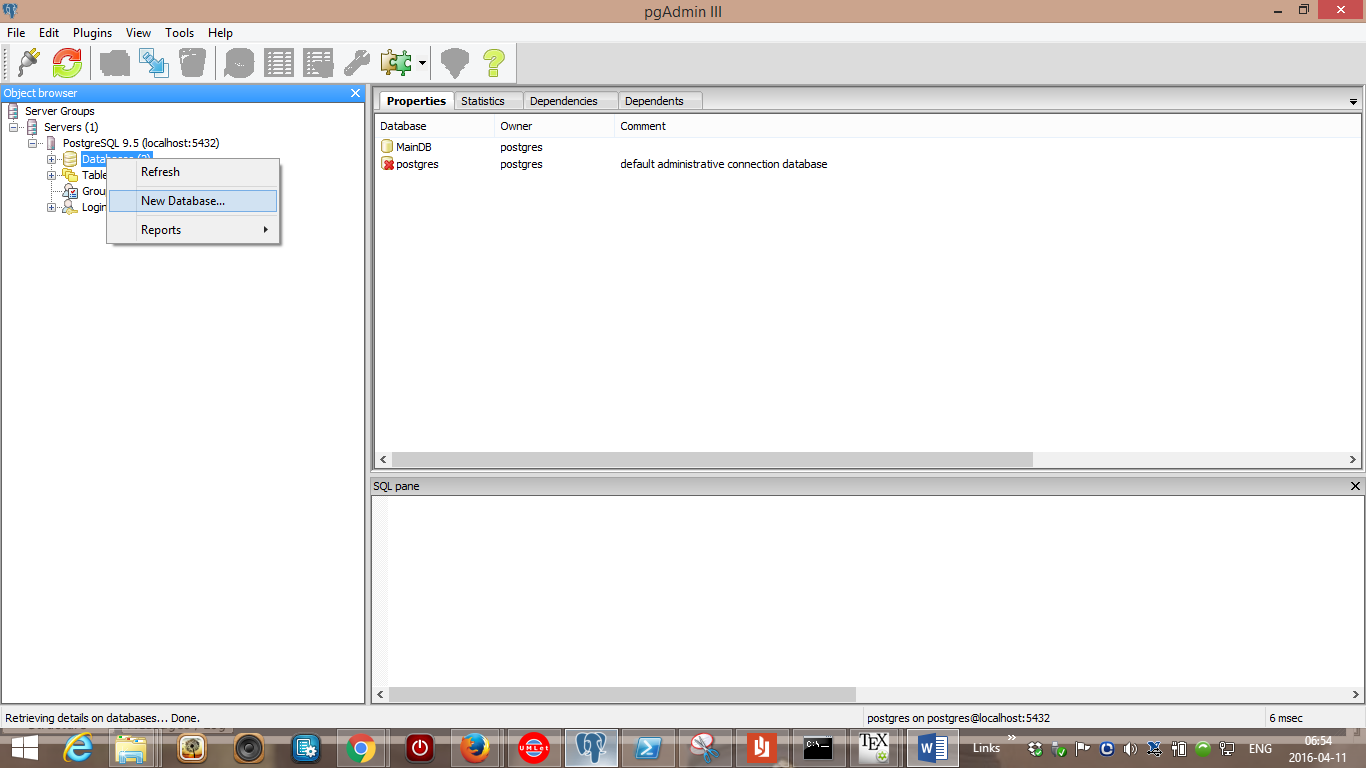
\includegraphics[width=3.5in]{pictures/postgresnewdb.png}
\caption{Creating a new database}
\label{DBCreation}
\end{figure}

\item under Name, type MainDB
\item click OK - a database is now created

\begin{figure}[hbt!]
\centering
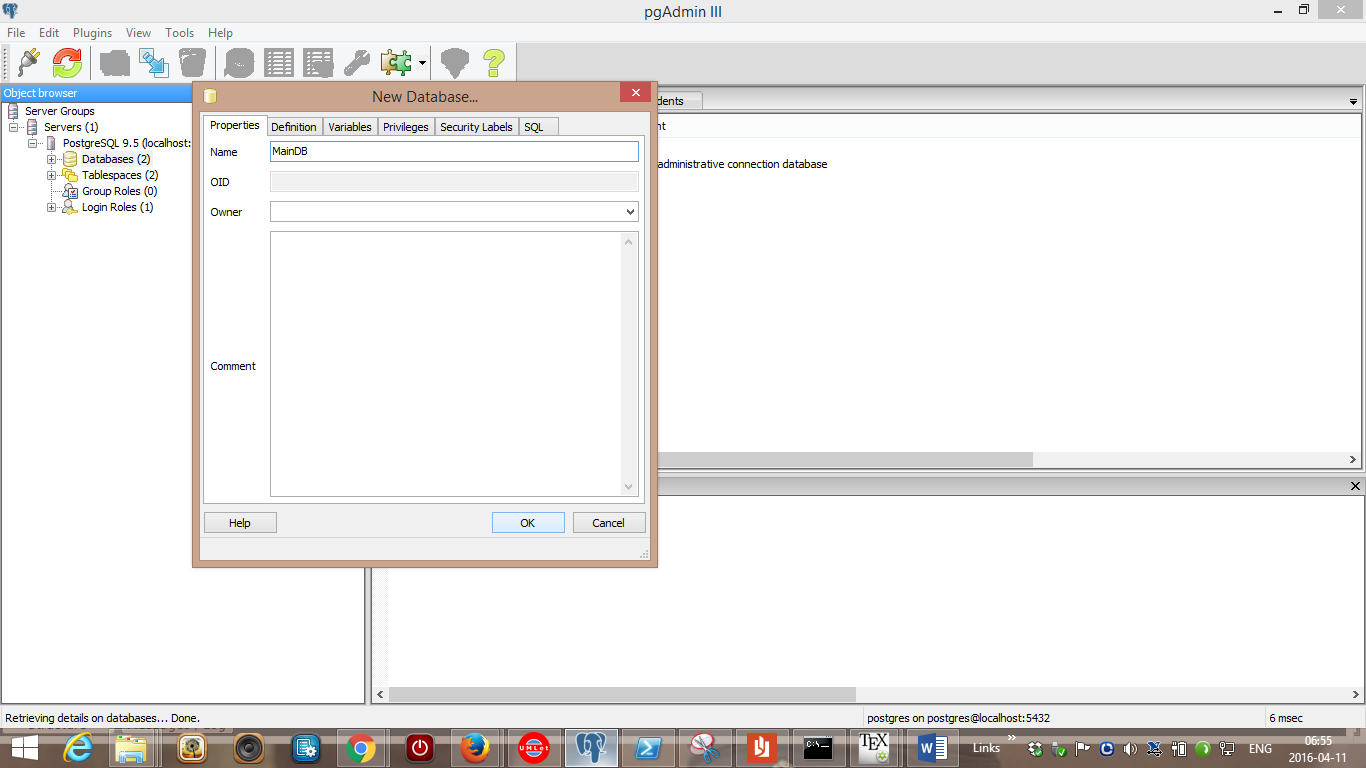
\includegraphics[width=3.5in]{pictures/postgresDBName.png}
\caption{Naming your new database}
\label{DbNaming}
\end{figure}

\end{itemize}
\end{itemize}





\subsection{Description of how to compile code}
\begin{itemize}
\item Go to the folder Project Submission/CourierJZ on the terminal
\item type : python createDatabases.py . The user has now added three tables to the MainDB created earlier.

\begin{figure}[hbt!]
\centering
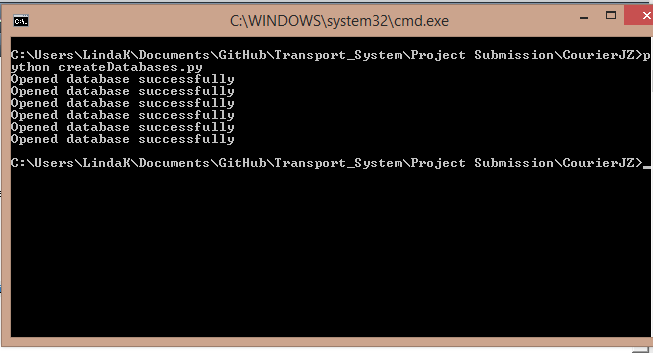
\includegraphics[width=3.5in]{pictures/createDbTerminal.png}
\caption{Creating databases}
\label{DbCreation}
\end{figure}

\item Go to the folder Project Submission/CourierJZ
\item open terminal in this location
\item type : python manage.py runserver . Django server is now running

\begin{figure}[hbt!]
\centering
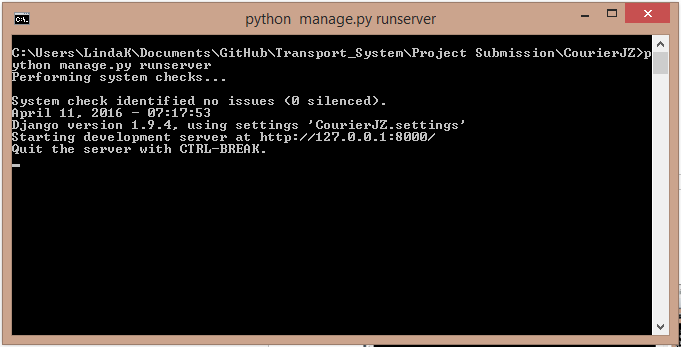
\includegraphics[width=3.5in]{pictures/runserver.png}
\caption{Running the server}
\label{Server}
\end{figure}

\item Go to browser (preferably Chrome). Type in 127.0.0.0:8000/courier/main
\begin{figure}[hbt!]
\centering
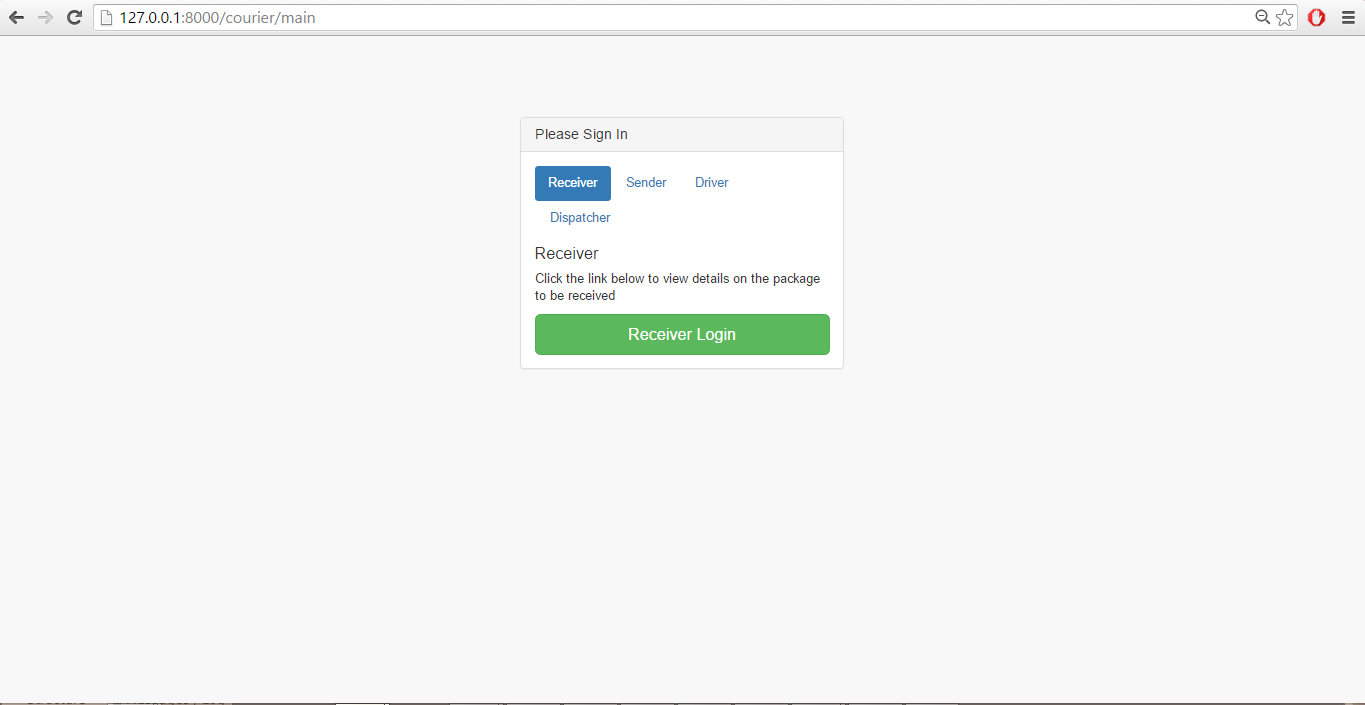
\includegraphics[width=3.5in]{pictures/mainpage.png}
\caption{The start page}
\label{StartMain}
\end{figure}


 

\end{itemize}

%\begin{align} 
%\begin{split}
%(x+y)^3 	&= (x+y)^2(x+y)\\
%&=(x^2+2xy+y^2)(x+y)\\
%&=(x^3+2x^2y+xy^2) + (x^2y+2xy^2+y^3)\\
%&=x^3+3x^2y+3xy^2+y^3
%\end{split}					
%\end{align}



%------------------------------------------------





%\paragraph{Heading on level 4 (paragraph)}
%
%\lipsum[6] % Dummy text
%
%%----------------------------------------------------------------------------------------
%%	PROBLEM 2
%%----------------------------------------------------------------------------------------
%
%\section{Lists}
%
%%------------------------------------------------
%
%\subsection{Example of list (3*itemize)}
%\begin{itemize}
%	\item First item in a list 
%		\begin{itemize}
%		\item First item in a list 
%			\begin{itemize}
%			\item First item in a list 
%			\item Second item in a list 
%			\end{itemize}
%		\item Second item in a list 
%		\end{itemize}
%	\item Second item in a list 
%\end{itemize}
%
%%------------------------------------------------
%
%\subsection{Example of list (enumerate)}
%\begin{enumerate}
%\item First item in a list 
%\item Second item in a list 
%\item Third item in a list
%\end{enumerate}
%
%%----------------------------------------------------------------------------------------

\end{document}